\documentclass{article}
\usepackage{hyperref}
\usepackage{pgfgantt}
\usepackage{graphicx}
\usepackage{caption}
\usepackage{amsmath}
\usepackage{microtype}
\usepackage{listings}
\usepackage{subcaption}

\graphicspath{ {./Images/} }

\begin{document}

\title{Advanced Computer Graphics}
\author{Oliver Eisenberg}
\maketitle
\tableofcontents

\section{Introduction}
Raytracing is a rendering technique that determines the visibly and colour of objects in a scene. The technique revolves around tracing rays, from the eye or camera, through each pixel and calculating the colour upon intersection with the closest object. The principles of raytracing can be extended to visualise shadows, reflection and transmission. 

\subsection{Visibility}
\subsubsection{Rays}
Rays are defined parametrically to take advantage of the \textit{t} parameter, this makes determining the object behind and closest to the camera straight forward - as a negative value means that the intersection occurred behind the camera.

\subsubsection{Ray Intersections}
To be able to add an object to a scene, it must support intersection tests with an arbitrary ray. As more complex objects, like a polymesh, use a series of smaller objects covering basic shapes, supporting these is enough to cover a majority of the meshes. The initial coursework code had sphere intersection support and was therefore expanded to include triangles and planes.
\subsubsection{The Camera}
The camera model allows the scene to be rendered around the viewer and is used to orientate the scene and emit rays. To be able to do this the camera requires knowledge of its position, where the camera is pointing, the up direction and distance to the image plane.
\subsection{Colour and Shading}
To determine the colour of the pixel that the ray was traced through, the closest object has to be identified. Therefore, all objects in the scene have to be iterated through before selecting the object. Furthermore the object has to be checked to see if is in shadow, this is done by emitting a shadow ray towards each light in the scene. Intersections found here, mean that the object is in shadow and, for that light source, the colour doesn't have to be calculated. 

\subsubsection{Local lighting}
Local lighting is the illumination of objects direct from the light source(s) in the scene. Objects can reflect lights either diffusly, shown in equation \ref{equ:diffuse}, which gives a matt effect, or specular - shown in equation \ref{equ:specular}, which acts like a mirror. 

\begin{equation}
I = I_lk_d(N.L)
\captionsetup{justification=centering,margin=0.5cm}
\label{equ:diffuse}
\end{equation}
\begin{equation}
R = I –2.0 \times (I.N) \times N
\captionsetup{justification=centering,margin=0.5cm}
\label{equ:specular}
\end{equation}

As surfaces are not perfectly smooth the Phong approximation \ref{equ:phong} was used, this gives an appropriate shine to an object.

\begin{equation}
I = I_lk_S(R.V)^n
\captionsetup{justification=centering,margin=0.5cm}
\label{equ:phong}
\end{equation}

Therefore the total colour calculation, per colour channel, for an ray to object intersection is:

\begin{equation}
I = I_ak_a + \sum I_{ln}(k_d(N.L) + k_s(R.V)^n)
\captionsetup{justification=centering,margin=0.5cm}
\label{equ:totalColour}
\end{equation}

Where,
\begin{itemize}
\item $ I_ak_a $ is the ambinent intensity and coefficent values
\item $ k_d(N.L)  $ is the diffuse coefficent, hit normal and incident light direction values
\item $ k_s(R.V)^n $ is the specular coefficent multiplied by the reflected ray and viewer direction to the power of n, the distribution controller whoes trypical values are around 20-200.
\end{itemize}

\subsubsection{Self Shadows}
When computing shadows self-shadowing can occur. This is caused by rounding errors, where, the shadow ray is generated at a starting point from within the original intersecting object. This causes the shadow ray to hit the inner object and declare that pixel as in shadow - even if it may not be. To resolve this issue the new shadow ray is shifted along the direction of the ray by a small amount. 

Testing all objects for shadows can be optimised as, for a single light source, once you found a shadow identifying another doesn't further shadow the pixel. Therefore the loop that checks for shadow can stop at the first occurrence. Further optimisations can be done through the use of a shadow cache. Shadow caching works due to ray coherence where if a ray is being emitted close by to a previously true shadow ray you can assume that ray also in shadow, preventing checking for an intersection.

\subsubsection{Global lighting}
Global lighting is the addition of secondary rays to compute mirror and transmissive surfaces. 

Reflection works by assuming a specular surface is a perfect mirror. Performing the equation \ref{equ:specular} and raytracing the result calculates the reflected colour. This is then added to the original colour calculated prior to reflecting. The cycle of ray generation for secondary rays leads to recursion. 

Similarly to reflection, transparency lends to recursion. This is because secondary rays are produced to simulate the movement of flight through a transparent object. To calculate refraction, the index of refraction needs to be set on object initialisation, this constant is used to determine how much the light is slowed by when entering the object. Depending on the incident angle and medium the refracting ray will either slow down and bend towards the normal, speed up and bend away from the normal or undergo total internal reflection. 
This, however, isn't realistic transparency. This is because, for real materials the angle of incidence changes the amount of reflection and refraction that will occur. To account for this the Fresnel equations (\ref{equ:fresnelkr} to \ref{equ:fresnelkt}) are applied. These result in more realistic behaviour.

\begin{equation}
r_{par} = \frac{(\eta cos\theta _i - cos \theta _t)}{(\eta cos\theta _i + cos \theta _t)}
\captionsetup{justification=centering,margin=0.5cm}
\label{equ:fresnelrpar}
\end{equation}
\begin{equation}
r_{per} = \frac{(cos\theta _i - \eta cos \theta _t)}{(cos\theta _i + \eta cos \theta _t)}
\captionsetup{justification=centering,margin=0.5cm}
\label{equ:fresnelrper}
\end{equation}
\begin{equation}
k_r = \frac{1}{2}\times\frac{(r_{par}^2)}{(r_{per}^2)}
\captionsetup{justification=centering,margin=0.5cm}
\label{equ:fresnelkr}
\end{equation}
\begin{equation}
k_t = 1 - k_r
\captionsetup{justification=centering,margin=0.5cm}
\label{equ:fresnelkt}
\end{equation}

\section{Raytracing Implementation}
The completion of lab sheets allowed to get familiar with C++ and to start building practical knowledge on raytracing. 

\subsection{Labs 1 \& 2}
Lab one and two allowed to build supporting functionality to use and test the implementation of raytracing. To be able to construct a wireframe, the line drawing function was updated to use an integer based approach using the Bresenhams Line Algorithm. The algorithm is an efficient method used to draw a straight line and avoids the use of floating point multiplication to draw pixels. Instead, Bresenham's algorithm increments axes so that the gradient of the currently drawn line remains similar to the goal gradient, where the goal is the initial vector from point A to B.

Lab two allowed the algorithm to be used to draw wireframes of an imported dataset. The given code in \textit{polymesh.cpp} was updated to be able to read 3D objects from \textit{.ply} files. There are several mesh data structures that can be used to store polymesh objects, the method supported in the \textit{polymesh.cpp} is the Shared Vertex(OBJ, OFF) where it contains an indexed list of vertices and faces (vertex indices). The teapot dataset is comprised of three header lines, these identify the number of vertices and faces that are contained and are iterated through to populate their respective vectors. The shared vertex data structure is adequate, however, more complex structures have the potential of reducing construction, query and improving efficiency. For example the \textit{.ply} file could have used Face-Based, which lacks in edge information, or Edge-Based connectivity, which excludes edge orientation information.

\begin{figure}[h]
\centering
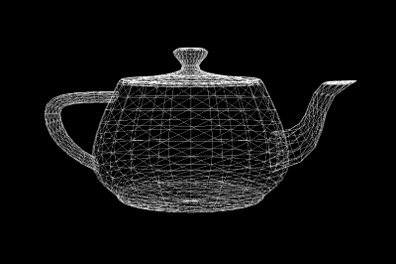
\includegraphics[width=0.5\textwidth]{wireframe}
\captionsetup{justification=centering,margin=0.5cm}
\caption{End product of lab two}
\label{fig:wireframe}
\end{figure}

\subsection{Lab 3 - Simple Raytracing}
\subsubsection{Framebuffer}
To be able to test triangle intersections could work through ray intersection tests, the rays were first tested on a depth buffer. The depth buffer uses the paramatric \textit{t} value in order to visualise the depth of the hit. By suppling the sphere intersection code this could be tested first here before developing and testing triangle intersections. The intersection testing for the sphere was straight forward using psudocode provided from the slides.

\subsubsection{Triangle intersection}
To compute triangle intersections the Möller–Trumbore algorithm was used. This was used instead of the method on the slides ~\cite{ref:lec04} anticipating the requirements for the barycentric coordinates to complete Gouraud shading further in the coursework. Baracentric coordinates allow for Gouraud shading as the values can be used to determine where on the triangle the intersection took place. Being able to follow the general intersection layout for spheres laid out the structure well for testing the triangles. The end result (figure \ref{fig:depthmap}) is shown, where darker surfaces indicate closer proximity to the camera.

\begin{figure}[h]
\centering
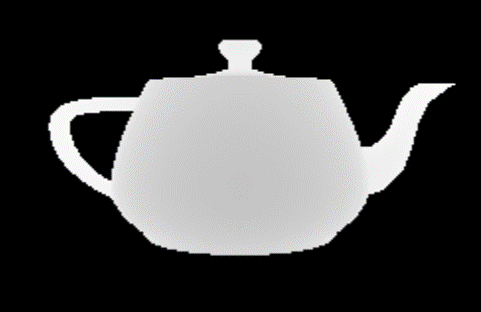
\includegraphics[width=0.4\textwidth]{depthmap}
\captionsetup{justification=centering,margin=0.5cm}
\caption{End product of lab three}
\label{fig:depthmap}
\end{figure}

\subsection{Lab 4 - Basic Lighting and Shadows}
Starting to work on lighting prompted further refactoring. In doing so, a scene class was created to create and store all the objects and lighting for the render. All lights belong to the base light class, this allows to predetermine shared variables and functions a light should have and for lights to be stored in a single vector.
\subsubsection{Types of light}
\subsubsection{Spot Lights - Directional lights}
Spotlights were first implemented due to their simplicity. Spotlights are considered to infinitely far from the scene and therefore have no position and all light rays are parallel.

\subsubsection{Point Lights}
The slides refer to two methods to create point lights, with and without an associated direction. As spot lights are directional, point Lights with a constant intensity were implemented. Allows a point light to be placed between objects to cast shadow outwards. This is demonstrated in figure \ref{fig:pointlight_white}. 
\begin{figure}[h]
\centering
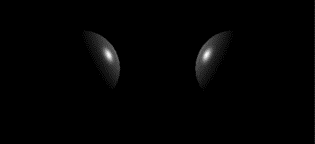
\includegraphics[width=0.5\textwidth]{pointlight}
\captionsetup{justification=centering,margin=0.5cm}
\caption{Simple render to illistrate pointlights}
\label{fig:pointlight_white}
\end{figure}

\subsubsection{Shadows}
Shadows are checked by sending a ray from the hit position to each light in the scene. If an intersection occurs the intensity from that light is removed. This allows for shadows of different intensity depending on the source. Originally the program would remove light intensity relative to the number of total lights - disregarding the light source's intensity. This was rectified and updated before the lab 4 submission date.

\begin{figure}[h]
\centering
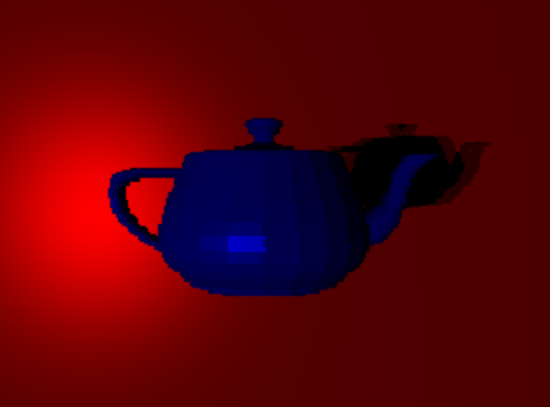
\includegraphics[width=0.5\textwidth]{teapotShadow}
\captionsetup{justification=centering,margin=0.5cm}
\caption{Teapot casting two shadows}
\label{fig:teapotShadow}
\end{figure}


In addition the shadow ray's length must be compared with the distance to the light, this is important as when adding planes to the scene a light source in between two planes can cause a shadow as if one of the planes obstructed the light. Instead the light ray is passing the source, therefore there would be no shadow, but then intersects with the secondary plane.

\section{Minor Optimisations}
\subsection{Colours \& Materials}
Originally objects had three intensity values representing the three primary colours in addition to the diffuse and specular coefficients. This was later updated to use a material and colour class. The colour class allowed for a collection of operations to be enabled, this was useful for adding and performing operations on colour. This change prompted the addition of materials now, instead of later in the coursework for textures to be applied. Materials were changed to hold specular, transmission values as well as the object’s base colour. This simplified the initialisation of objects in my scene class to creating several materials for objects to use.

Furthermore, by splitting intensity into colours it allows the addition of coloured lights and control over what coloured objects can reflect this could also benefit possible diffraction and iridescence rendering.
\begin{figure}[h]
\centering
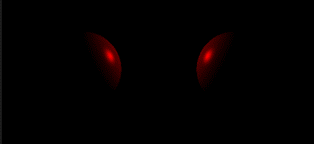
\includegraphics[width=0.5\textwidth]{pointlight_redlight}
\captionsetup{justification=centering,margin=0.5cm}
\caption{Simple render like figure \ref{fig:pointlight_white} but with a red light}
\label{fig:pointlight_red}
\end{figure}

\section{Photon Mapping}
Photon mapping is a two pass algorithm that allows to compute global illumination, caustics and precipitation media, building on raytracing. In the real world most light is indirect, a standard raytracer cannot simulate interreflection between diffuse surfaces. The combination of BRDFs and the Rendering Equation provide a way to model photon paths in the correct direction.

\subsection{The rendering equation}
\begin{equation}
L(x',\omega) = E(x',\omega') + \int\rho_x'( \omega,\omega') L(x,\omega)G(x,x')V(x,x') dA
\captionsetup{justification=centering,margin=0.5cm}
\label{equ:fresnelrpar}
\end{equation}
The equation comprises of five terms, unless the object is not emissive. If the object is emissive then $ E(x',\omega') $ is the emitted radiance from a point, otherwise it is 0. The other four terms describe the how the radiance of other objects in the scene contribute at the point.

\begin{enumerate}
\item $ \rho_x'( \omega,\omega') $ describes the contribution from the reflectivity (BRDF) from the other object. 
\item $ L(x,\omega) $ is the radiance from the other object.
\item $ G(x,x') $ is the geometric relationship between the two surfaces.
\item $ V(x,x') $ is the visibility of the other object. The equation should only apply to the closest object, therefore it resolves to 0 if the object is obstructed.
\end{enumerate}

This models other techniques like raytracing and radiosity but doesn't support all natural lighting features, for example refraction and caustics.

\subsection{BRDFs}
Bi-directional Refectance Diribution Functions are a method to specify the amount of light that leaves in relation to the light that arrived. The ambient, diffuse and specular models used when raytracing fit the functions. BRDFs are four dimensional and more parameters can allow for more complex materials. For example adding wavelengths will allows to model Iridescence. 

\subsection{Two pass algorithm}
\subsubsection{Pass one}
In the first pass, two photon maps are generated with different purposes. One is for high resolution caustic photons and a lower resolution general one ~\cite{ref:lec12}. Similarly to raytracing photons are traced through the scene and for each photon hit, type, directional, positional and colour information is stored and, if a secondary photon can be generated from reflection follow and recurse. This process is repeated for all n photons. The photon information is stored in a balanced kd-tree, which is a special case of a binary search tree.

When a photon does hit a surface Russian roulette is used ~\cite{ref:photonMappingGUIDE} to determine what outcome to choose. The probability for each outcome is calculated using the hit object's diffuse, specular and transmissive values. 
\begin{lstlisting}[language=c++]
r = generate_random[0, 1];
if (0 <= r && r < diffprob) 
// diffuse reflection
if (r < diffprob+specprob) 
// specular reflection
if (r < diffprob+specprob+transmissiveprob) 
// transmissive calculation
if (r < 1)
// absorb
\end{lstlisting}

A Caustic map is created by emitting photons towards specular surfaces only, these photons are stored when they hit a diffuse surface and can be rendered directly as a radiance estimate.

\subsubsection{Pass two}
Rendering is done using raytracing but with the knowledge from the photon information gathered. Accurate or approximate calculations can be done at each intersection. The accurate method is the normal raytracing method and is used for direct illumination and specular reflections. The approximate uses the radiance estimate is used for everything else. 

\begin{enumerate}
\item Direct : Either accurately or approximately 
\item Specular : Normal Monte Carlo raytracing
\item Caustic : Render caustic photon map directly
\item Soft indirect : approximate is included in the global photon map, accurate can be done using importance sampling
\end{enumerate}

\section{Photon Tracing Implementation}
Some difficulty was encountered when choosing a library that supported kd trees. This was because they were often static libraries which made integration harder on a windows subsystem for Linux. This heavily influenced the chosen library to handle KD Trees. The library chosen \textit{Alglib} ~\cite{ref:alglib} was created to be added to code like your own classes where you include the relevant headers and compile the \textit{.cpp} files yourself. The library's documentation was enough to create a local wrapper class that allowed easy access when storing and accessing photon from their maps.

\subsubsection{Random emission - Lighting}
Lights had to updated with relevant random emission direction and position functions. My point light was therefore changed so that all random points started from the point light's position and a random direction could be generated. This behaviour could not be generalised as for spot light the points would have to randomly start in different positions but have the same direction vector.

\subsubsection{Specular \& Gloss}
This was straight forward to implement as it is rendered using standard raytracing techniques that were developed during the lab hand-ins. 

\subsubsection{Caustics}
Caustics are computationally intensive to calculate using standard raytracing methods but was straight forward to implement using a separate caustic photon map. In a caustic map photons are emitted from the light source to reflective and transmissive objects only, this was done by tracing photons to random positions to supportive objects. Later when rendering, the map is calculated using a radiance estimate. A caustic map can be filtered prior to rendering to smooth out hard edges, however the caustic renders I was generated never seemed to be extremely hash - this may have been due to a high nearest neighbour count in my caustic photon map.

\begin{figure}[h]
\centering
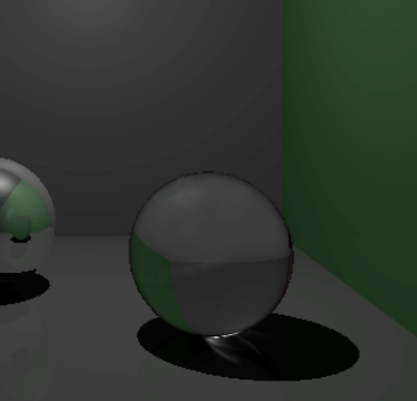
\includegraphics[width=0.4\textwidth]{caustics}
\captionsetup{justification=centering,margin=0.5cm}
\caption{Render with caustics}
\label{fig:caustics}
\end{figure}

\subsubsection{Indirect soft diffuse}
During the rendering process, after raytracing if the object's material is reflective or transmissive, rays are diffusely reflected of the intersecting object. This allows for the visualisation of colour bleeding. This was done by tracing a diffusion ray until intersection, at that point - depending on accuracy preference the value was obtained from the global photon map directly or by sampling.

I attempted to render everything accurately, including indirect diffuse reflections - even though inaccurate was suggested unless it could not be performed. Unfortunately the results of attempting to accurately render the soft diffuse resulted in high amount of noise, as shown in figure ~\ref{fig:indirectdiffonly} and subfigure ~\ref{fig:sub1} as a whole scene. To reduce the noise the image was passed through a gaussian low pass filter, the result of this are shown in subfigure ~\ref{fig:sub2}. Unfortunately this don't produce the desired effect, I therefore decided to examine the difference between inaccurate and the use of both inaccurate and accurate to render the scene. This is shown in figure \ref{fig:AccuratefilterComp}. 

\begin{figure}[h]
\centering
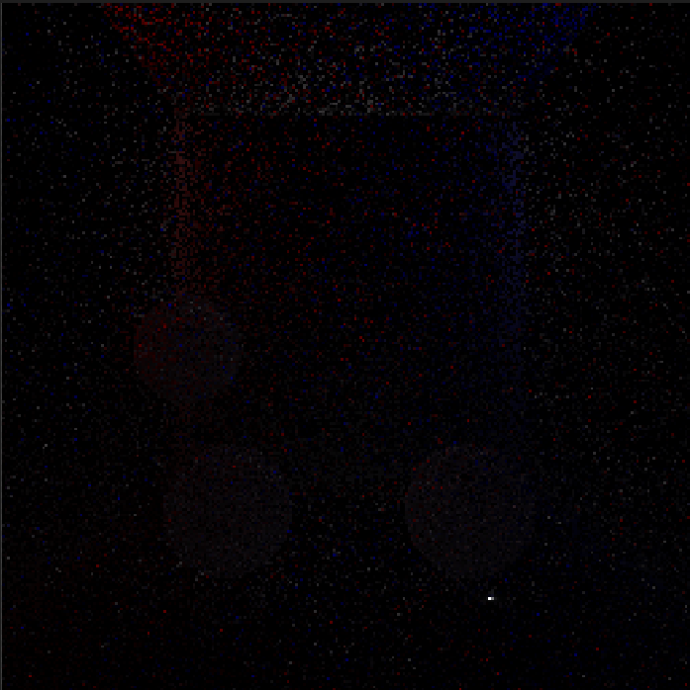
\includegraphics[width=0.65\textwidth]{indirect_softdiffuse_accurate}
\captionsetup{justification=centering,margin=0.5cm}
\caption{Render showing indirect soft diffuse only}
\label{fig:indirectdiffonly}
\end{figure}

\begin{figure}
\centering

\begin{subfigure}{.5\textwidth}
\centering
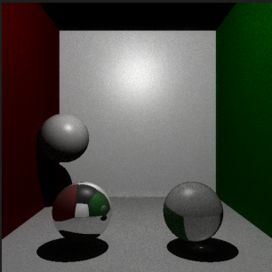
\includegraphics[width=0.85\linewidth]{accurate_sft_diff_RAW}
\caption{Acurrate soft diffuse}
\label{fig:sub1}
\end{subfigure}%
\begin{subfigure}{.5\textwidth}
\centering
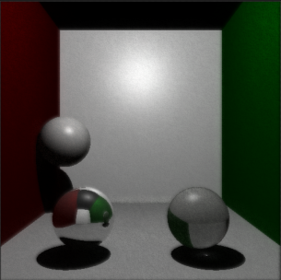
\includegraphics[width=0.85\linewidth]{accurate_sft_diff_FLT}
\caption{Accurate soft diffuse - filtered}
\label{fig:sub2}
\end{subfigure}

\caption{Before and after filtering accurate soft diffuse}
\label{fig:AccuratefilterComp}
\end{figure}

\begin{figure}
\centering

\begin{subfigure}{.5\textwidth}
\centering
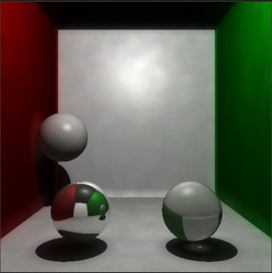
\includegraphics[width=0.85\linewidth]{inaccurate_sft_diff_RAW}
\caption{Inacurrate soft diffuse}
\label{fig:sub3}
\end{subfigure}%
\begin{subfigure}{.5\textwidth}
\centering
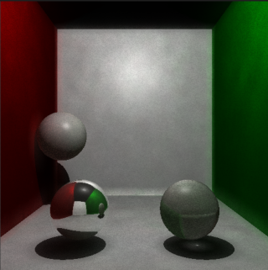
\includegraphics[width=0.85\linewidth]{comb_sft_diff_RAW}
\caption{Combined soft diffuse}
\label{fig:sub4}
\end{subfigure}

\caption{Scene comparison using different soft diffuse calculations}
\label{fig:AccuracyComp}
\end{figure}

Overall I am undecided which scene I prefer, \ref{fig:sub3} is very clean, however, \ref{fig:sub4} seems to have slightly more colour bleeding and the low level noise gives the scene a nice metallic texture. Therefore I decided to use both methods when rendering the scene. To sample a position, the surrounding photon hits were collected and a subset were reversed and their radiance calculated using their originating position , this would only happened to indirect photons otherwise you may sample colours on opposite walls from a central light source unintentionally.


\newpage
\begin{appendix}
\listoffigures
\end{appendix}
\bibliographystyle{ieeetr}
\bibliography{./Bibliography}

\end{document}


